\chapter{Аскольдова могила}

Прежде писали – «на живописных склонах Днепра», ныне это звучит натянуто. Тогда просто. Есть на склонах Днепра урочище Аскольдова могила. Под нею обычно понимают храм с ротондой:

\begin{center}
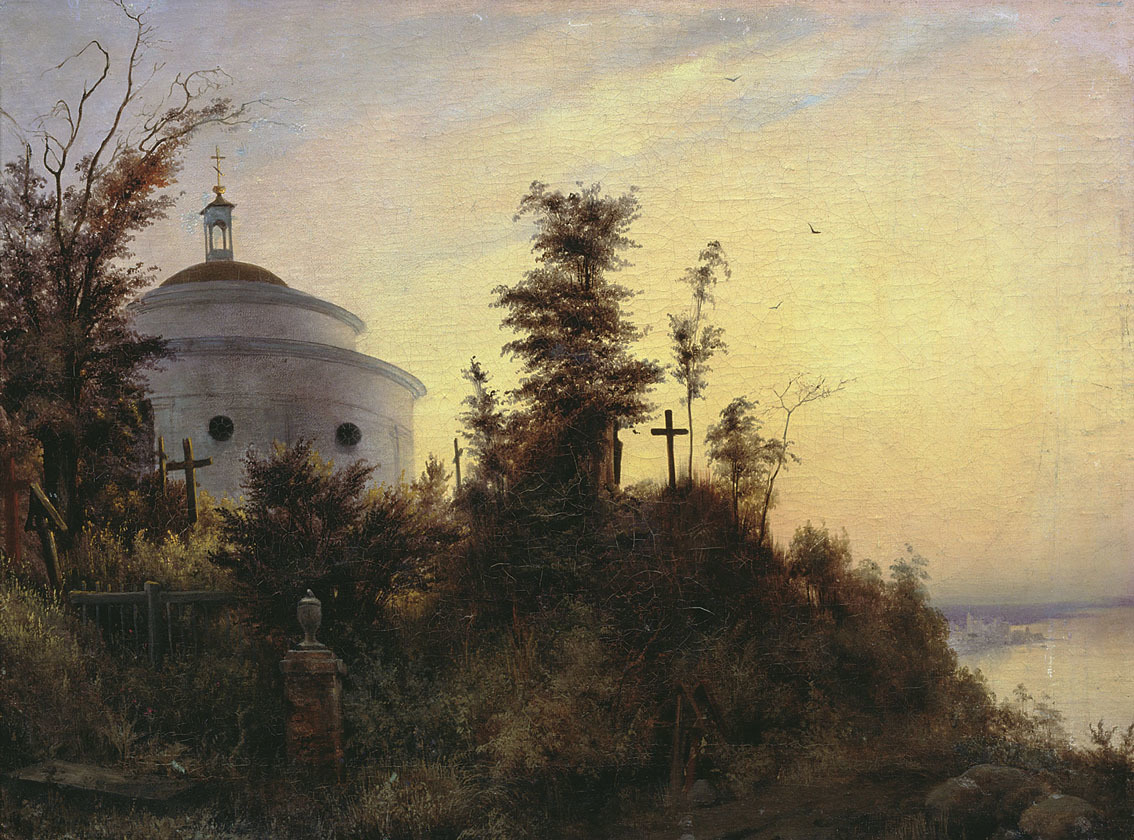
\includegraphics[width=\linewidth]{chast-volga/oskoldidir/ascoldova_mogila_1837.jpg}

\textit{ШтернбергВасилий Иванович, Аскольдова могила, 1837.}
\end{center}

Раньше на месте этой кладбищенской церкви стояла другая, деревянная. В 1810 году её заменили новой, каменной, но тоже святого Николая, как повелось издавна от бытовавшего тут одноименного монастыря. Круглая, с колоннами, по проекту архитектора Меленского она была возведена средствами воронежского городского главы Самуила Никитича Мещерякова в память своей усопшей о 1808 году в Киеве жены Александры, которая была тут же, на Аскольдовой могиле, погребена. Кладбище упразднили в 1840 году, впрочем без разрушения, да и хоронить продолжали понемногу.

\begin{center}
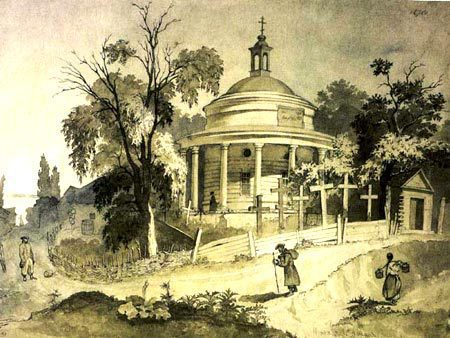
\includegraphics[width=\linewidth]{chast-volga/oskoldidir/shevchenko_am.jpg}

\textit{Тарас Шевченко, Аскольдова могила, 1846, сепия, акварель.}
\end{center}

В новой церкви было два яруса – наземный и подземный, что служил для захоронений, в частности людей, чьими денежными стараниями церковь возводили и обустраивали. В 1840-х храму грозила гибель, место его вовсе хотели срыть – приближался прокладываемый Николаевский спуск. Уже тогда для устранения неугодных строений использовали предлог – объект в аварийном состоянии, ценности не представляет – и церковь собирались снести именно под таким соусом. Но царь Николай I, заботящийся более о довольной жизни зданий, нежели поэтов, предотвратил разрушение фразой, написанной на бронзовой доске внутри церкви: «Ничуть падением не грозит – немного нужно поправки и церковь должна стоять». Это был ответ инженерам, которые из-за трещины на стенах предлагали разобрать всё.

В 19 веке над западными дверьми была надпись: «На сем месте тайно церковь существовала устроенная христианами от Андрея Первозваннаго апостола просвещенными». Что послужило основанием к надписи и стоит ли доверять ей, неведомо.

\begin{center}
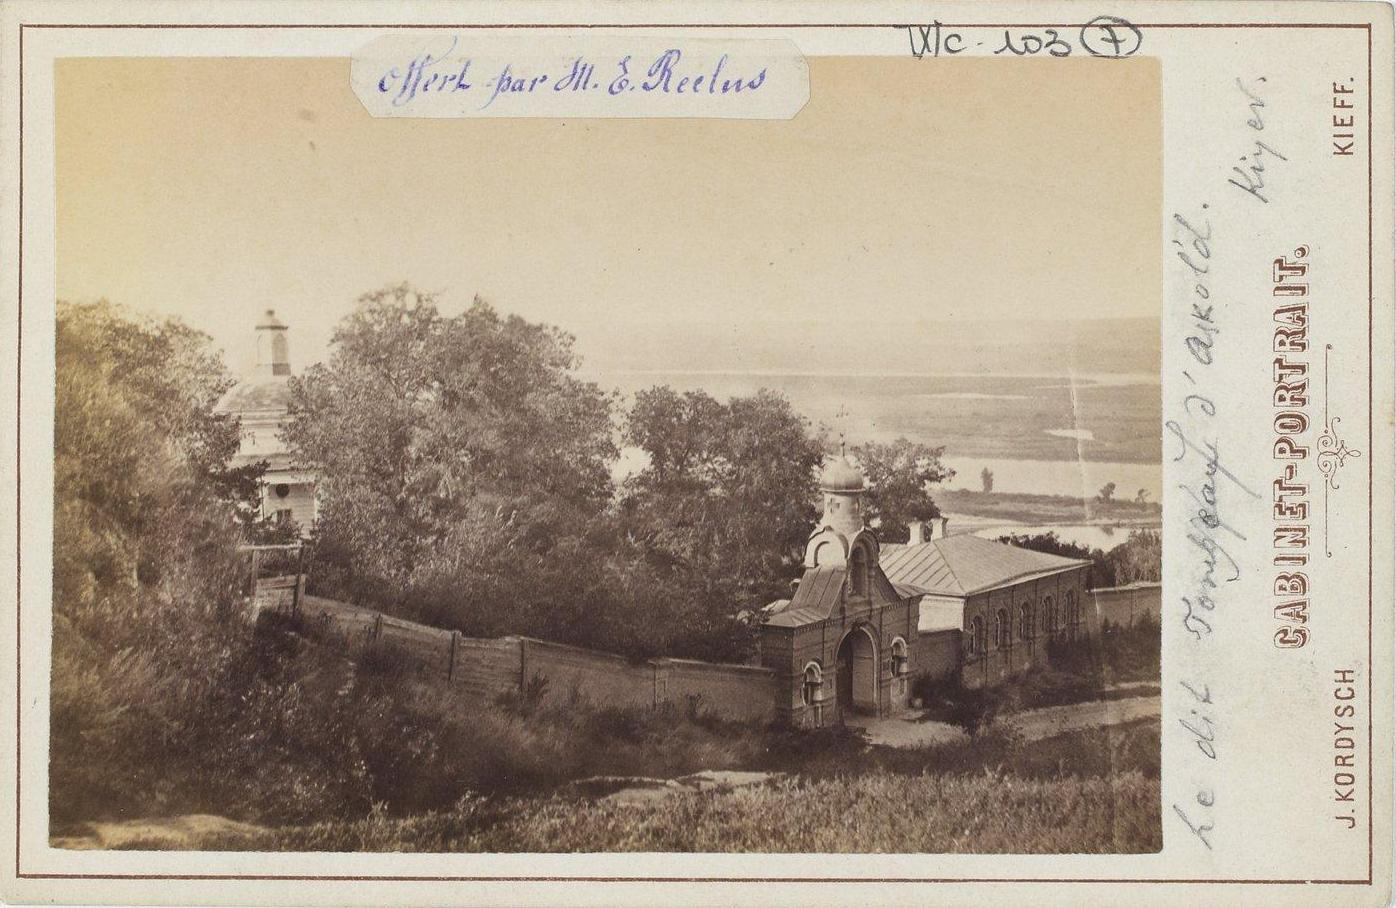
\includegraphics[width=\linewidth]{chast-volga/oskoldidir/amog.jpg}

\textit{Дореволюционная открытка.}
\end{center}

В 1935 году кладбище, насчитывающее около двух тысяч могил, уничтожили. Часть известных захоронений перенесли на другие кладбища. Например, прах летчиков-асов Нестерова и Крутня теперь покоится на Лукьяновском. А вот куда девали кости Меринга, Соловцова и тысяч других? Подозреваю, их оставили в земле, снеся надгробия. Вокруг церкви обустроили парк. Живые люди отличаются от покойников проявлением деятельности в нашем мире. Деятельность имеет два противоположных направления – создание и разрушение.

Особо старался в разорении киевских кладбищ Владимир Затонский, работая в 1922-1924 и 1933-1938 годах народным комиссаром просвещения УССР. Щекавицкое, часть Байкового, кладбище на Замковой, Кирилловское и так далее. Вот распоряжение Затонского председателю Киевского горсовета Александру Гинзбургу:

\begin{quotation}
По моему поручению комиссия археологов и художников осмотрела Аскольдову могилу. Как мы с вами условились, Аскольдову могилу как кладбище нужно ликвидировать, церковь – закрыть. Надгробные памятники использовать как материал для строительства и оформления парков и т.д. Одно лишь замечание – желательно, чтобы мрамор в больших кусках был использован как материал для скульптуры, а то, к примеру, не могли до последнего времени найти куска белого мрамора, чтоб заказать бюсты вождей революции. 3.ХI.1934. Подпись.
\end{quotation}

И мрамор таки передали – студентам Художественного института, а металлические ограды отправили в металлолом.

Буйноволосый сын волостного писаря из села Лысец, Подольской губернии, лучше бы Затонский оставался преподавателем физической химии в Политехе, или, как в юношестве, прыгал с места на стол, нежели войдя во власть подписывал смертные приговоры древним кладбищам и соборам. Но и ему, верному ленинцу, был вынесен приговор в 1938-м. А всего четыре года до того, на Затонского обрушилась лавина писем по поводу предстоящего сноса Михайловского собора. Ведь в Киеве, в рамках сооружения правительственного центра, после проведения конкурса, задумали вот что – два одинаковых здания со стометровым памятником Ленину точно над Боричевым увозом.

%\begin{center}
%\includegraphics[width=\linewidth]{chast-volga/oskoldidir/mihayl.jpg}

%\textit{Проект Иосифа Лангбарда.}

%\end{center}


\begin{center}
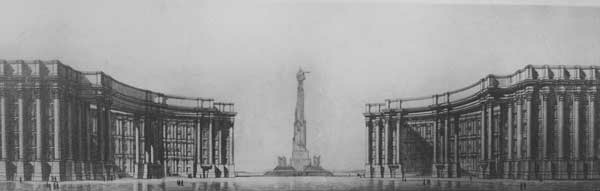
\includegraphics[width=\linewidth]{chast-volga/oskoldidir/langbard1.jpg}

\textit{Проект Иосифа Лангбарда – вид со стороны Михайловской площади.}
\end{center}

\begin{center}
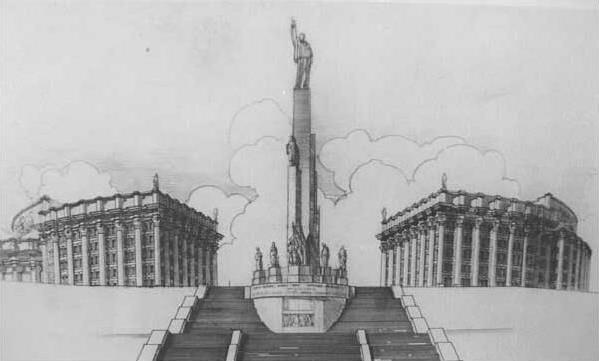
\includegraphics[width=\linewidth]{chast-volga/oskoldidir/langbard2.jpg}

\textit{Проект Иосифа Лангбарда – вид со стороны Днепра.}
\end{center}

Из задуманного построили лишь здание ЦК КП(б)У слева (теперь там МИД), однако под проект снесли и Михайловский собор, где хотели возвести здание Совнаркома.

И вот 1934 год, еще не приступали. Академик Затонский пишет 11 июня Письменному, члену созданной для сноса комиссии\cite{mikorsky01}:

\begin{quotation}
Т. Письменный! ІІо поводу Михайловского собора любители старья подымают шум, будто там на стенках (частью на виду, частью в замазанном виде под слоем штукатурки) имеются картины (мозаика, фрески). Я направил в Киев нашего заведывающего Музейным отделом т. Макаревича с тем, чтобы он без шуму организовал обследование, поковырял где надо стенки и т.п. Это придется делать с привлечением кое-кого из спецов. Заодно они должны прикинуть, каким образом производить съемку стенной живописи, которая действительно представляет художественно-историческую ценность. 

Музейщики\footnote{Переправлено со «всякие музейные старьевщики».} будут, разумеется, тянуть волынку. В этом деле в дальнейшем нам придется разбираться вместе с Всеволодом Аполлоновичем\footnote{Балицким, комиссаром госбезопасности.}. Сейчас Вы примите участие в том, что поручено предварительно подработать т. Макаревичу.

В частности, т. Чердак может быть полезен по части подбора и характеристики подходящих ученых спецов.

Привет. В. Затонский.
\end{quotation}
 
«Любители старья» – ученые, да и просто неравнодушные люди из Москвы и Ленинграда, возмутившиеся грядущим сносом собора. Феликс Кон, заведующий музейным отделом Наркомпроса РСФСР, вступил с Затонским в переписку и предлагал сохранить храм. Затонский же соглашался только на снятие фресок, и очень с этим спешил. Строительство тормозят!

13 июня Затонский написал в Москву, Бродскому – президенту Академии Художеств. Просил выслать специалистов для снятия фресок. И в тот же день, Затонский в письме к Кону сетовал, что московские специалисты – не помогают. Они еще не прибыли, Бродский еще не читал письмо киевского академика, но зловредные москвичи уже не помогают!

\begin{quotation}
Имею из Киева сведения, что уважаемые специалисты из Художественной Академии не помогают в организации снятия фресок и мозаик с Киевского Михаиловского собора, а наоборот затягивают дело...

Тем временем ученые любители старья всячески добиваются, как это Вы знаете из писем, которые Вы же мне переслали, сохранения собора в целости. Поскольку Вы этим делом интересуетесь, сообщаю, что вопрос о сносе собора решен. Может идти лишь речь о снятии мозаик и фресок. Чем дольше будут канителить, тем меньше останется времени для этой сложной операции. Может кончится тем, что придется ограничиться лишь фотосъемками. Виноваты будут сами старьевщики. Ежели этим по-прежнему интересуетесь, нажмите на Академию Художеств, разъяснив им положение дела.
\end{quotation}

«Любители старья», «старьевщики». Как горько повезло Киеву.

Трехсвятительскую церковь, что стояла неподалеку на месте Перунова кумира и прочих идолов, Затонский снес, по его выражению, «без канители». При нем же, один за другим, уничтожили другие древности – давнюю колокольню Кирилловской церкви, церковь Петра и Павла (бывшая доминиканская катедра), мощнейший Николаевский Слупский монастырь (окрестности Дома пионеров, рядом с площадью Славы), Братский монастырь, Успенский собор на Подоле (его потом возродили и утверждают, что это «Пирогоща»), Рождественскую церковь на Почтовой площади, Николы Доброго.
 
Затонского увековечивали еще прижизненно в названиях улиц, потом, как водится, их переименовывали, но посмертная реабилитация и восстановление в партии, при Хрущеве, дали имени новую жизнь – улицы имени, учреждения имени... В Киеве до 1991 года была улица Затонского (теперь Михаила Донца), висят мемориальные доски на главном корпусе Политеха и на стене Гуманитарного корпуса универа Шевченко. Забыли на здании Верховного совета соорудить – там стоял особняк, где жил Постышев, а во дворе флигель занимал Затонский. Не так уж далеко от Николаевского монастыря и Аскольдовой могилы.

Советские граждане помнят там колоннаду на крыше церкви, как бы второй наземный этаж – её надстроили в том же 1935 году и в здании разместился ресторан, а потом оно использовалось как парковый павильон, например для проведения выставок.

Бывший член академии наук УССР, Микорский в эмиграции выпустил работу «Разрушение культурно-исторических памятников в Киеве в 1934-1936 годах»\cite{mikorsky01}, где писал:

\begin{quotation}
[...] приходилось слышать, что на Аскольдовой могиле под ротондальной часовней был обнаружен склеп. Свод был пробит, и в склепе была якобы найдена каменная гробница со скелетом. Трудно сказать, была ли это та гробница, которая приписывалась князю Аскольду, или какая-либо иная.
\end{quotation}

Но мы знаем, что подземный этаж в 19 веке служил для погребения людей, пожертвовавших церкви немалые деньги. Идет ли речь об одном и том же помещении?

Во время Великой Отечественной войны местность снова стала кладбищем. До сорок четвертого года немцы хоронили там своих, а затем наши – солдат Красной армии, погибших при освобождении Киева. В 1957 году эти, отечественные захоронения были перенесены в Парк Вечной Славы, туда, где мемориал с Вечным огнем. В 1992-м церковь отдали Украинской Греко-Католи\-ческой Церкви, а в 1997 или 98 году верхнюю колоннаду сняли. Относительно недавно около церкви приладили табличку, мол, тут – памятник археологии «Культурный слой села Угорское», датированный 10-13 веками. Но летописи молчат о таком селе. А еще в статьях любят писать, что-де около Аскольдовой могилы, в 1853 году в «во время археологических раскопок» нашли религиозную пещеру с фресками, и что это там постриглась в монахини мать Феодосия Печерского. Ошибка на ошибке.

\newpage
\vspace*{\fill}
\begin{center}
\includegraphics[width=\linewidth]{chast-volga/oskoldidir/\myimgprefix a01.jpg}
\end{center}

\begin{center}
\includegraphics[width=\linewidth]{chast-volga/oskoldidir/\myimgprefix a04.jpg}
\end{center}
\vspace*{\fill}
\newpage
\vspace*{\fill}
\begin{center}
\includegraphics[width=\linewidth]{chast-volga/oskoldidir/\myimgprefix a03.jpg}
\end{center}

\begin{center}
\includegraphics[width=\linewidth]{chast-volga/oskoldidir/\myimgprefix a05.jpg}
\end{center}
\vspace*{\fill}
\newpage

\begin{center}
\includegraphics[width=\linewidth]{chast-volga/oskoldidir/\myimgprefix a06.jpg}
\end{center}

Пещеру отрыли, в самом деле, 25 мая 1853 года, когда прокладывали дорогу к Цепному мосту – но гораздо южнее Аскольдовой могилы. Под Берестовым начали срывать отвесный холм, мешавший дороге (известной теперь как Днепровский спуск) – и при разрушении склона нашли пещеру. Более чем подробно её положение дает Каманин в книге «Зверинецкие пещеры». %Некоторые исследователи считают пещеру возле спуска той самой варяжской пещерой, которую «обрёл» Антоний, придя на Берестове.

Каманин называл открытую пещеру Никольской (отмечая её сходство со Зверинецкими пещерами в устройстве), Закревский – «Ивановой пещерой и Цепного моста», Срезневский – «пещерой Ивана-Грешника и Феофила», Антонович – «пещерой у Цепного моста». В 1840-х её, во время ремонта крепости, тоже откапывали, а потом засыпали. В 1853 году пещеру осмотрела ученая комиссия, зарисовали надписи на стенах: «Ивано, грешный, седе жил есть», «Иванов гроб печерника», «Господи, помози рабу своему Феодосеви и Феофилови. Аминь», «Многа лета». 

Найдены изображения крестов, лика некоего святого – решили, что это Николай-чудотворец. Деревянная доска, возможно от гроба «Ивано», ибо на ней была надпись: «Ивано» и шестиконечный крест. Каманин предположил, что именно в эту пещеру удалялся Феодосий Печерский по время Великого поста.

В печать попало несколько статей, и – всё, след теряется. Пещеру засыпали в том же году.

Учитывая близость описываемой местности к Лавре и тамошним пещерам, можно предположить связь с последними.

Вернемся к Аскольдовой могиле. В тех краях, под землей находится обширный комплекс дренажно-штольных систем для отвода грунтовых вод, известный среди диггеров как «Аскольдовка». Холм изрыт изрядно – интересно, проводились ли при этом археологические исследования?
 
%\begin{center}
%\includegraphics[width=\linewidth]{chast-volga/oskoldidir/ijakevich-oscold.jpg}

%\textit{Иван Ижакевич, Аскольдова могила, первая половина 20 века}
%\end{center}

Считается, что на месте Аскольдовой могилы похоронен Оскольд, он же Аскольд. Его с соратником Диром часто величают князьями, хотя оба деятеля были убиты именно по обвинению, что не княжеского роду, а в Киеве княжат! Многие списки упорно отрицают их княжеское происхождение.

В большинстве известных источников, Оскольд всегда соседствует с Диром. Оба одновременно правили Киевом. С давних времен могила Оскольда якобы известна, а могила Дира затерялась. Пишу «якобы» вот почему. Языческая могила Оскольда – это курган. А покажите мне там, на склонах Днепра под дворцом пионеров, хоть один уцелевший курган! В обозримом по источникам прошлом есть только церковь в урочище Аскольдова могила, и церковь эта по летописному преданию стоит на месте кургана или поблизости.

Кто такие Оскольд и Дир? У Нестора хрестоматийного про них сказано – были «мужами знаменитыми» при Рюрике, а согласно некоторым спискам – мужами у Вещего Олега, или вообще сами по себе. Варяги. Или не Варяги, а племянники Кия. Хотя в одном списке Оскольд и Дир убивают Кия, Хорива и Щека. Сплошные противоречия! Гиляров выписывает\cite[стр. 114]{gilyarov01}:

\begin{quotation}
посадниками Новагорода страна та управлялась, дондеже во Кривичах и Древлянах по некоем их князе, имянем Кия, от него же и град создан бысть Киев, обладаху племянники его Осколд и Дир и насиловаху Словяном, иже в Великом Новограде.
\end{quotation}

По более известным спискам, Оскольд и Дир отпросились у Рюрика, «с родом своим» идти к Цареграду, от Смоленска вдоль течения Днепра. Добрались до Киева, спрашивают у населения: «Чей есть град сей»? В ответ местные, будто справочное бюро: «Были три брата, Кий, Щек и Хорив, которые построили град сей и померли давно, ныне владеют нами Казары, им дань платим».

Каким образом Оскольд и Дир вывели Киев из подданства Козарам, летопись умалчивает. Будто не было ни дани Козарам, ни местной власти.

Оскольд и Дир спокойно оседают в Киеве, «умножают Варягов» и правят окрестными землями, воюя с Древлянами и Угличами. Болгары (балканские или волжские?) убивают сына Оскольда.

Сейчас мы вступим в мутные воды датировок, где дно, основа, сокрыта от глаз, и приходится шарить ногой, натыкаясь на подводные ямы.

Если вы легкомысленно читаете эту книгу случайным образом, вернитесь почти в самое начало, к главе «Летописание и летосчисление», где я подробно объясняю, почему не доверяю летописным датам, как устроен счет годам в летописях и как этот счет отличается от списка к списку.

Общепринятая датировка – средство для убаюкивания совести науки. Далее я буду, однако, использовать «научные» даты, чтобы проявить возникающие при этом нелепости. Да и чертовски привычно видеть исторические сведения с четкой привязкой к годичной шкале.

В 866 (6374) году, по летописям, Оскольд и Дир скопив силы идут войной на Греков, на Царьград. Плывут морем. Дошедшая до нас Повесть временных лет именует Оскольда и Дира, и войско их – Русью, подчеркивая родство с народом Рюрика и Вещего Олега. Между тем Кий, Хорив и Щек, по Нестору – Поляне, не Русь. Но кое-какие списки говорят про поход Оскольда на Царьград: «Оскольд с Поляне».

Заметим также, что если Кия в Царьграде принимали с великой честью и кажется мирно, то Оскольд с Диром не поддерживают с Византией дружеских отношений, идут войною.

Правитель Царьграда, Михаил – или, как его величает история, император византийский Михаил III (842–867) – прославился устроением на пирах соревнований пердунов. Но во время нападения Русов сражался с Сарацинами, был вне своих владений. И покуда спешно возвращался, Оскольд и Дир устроили бойню около Царьграда, порешили множество Греков-христиан, и затем осадили город двумя сотнями лодей.

Михаил с трудом пробился в город, и купно с патриархом Фотием исправил положение – пошел в церковь святой Богородицы во Лахернах, молился ночь напролет, потом взял ризу Богородицы и отнес в пролив, где оную ризу омочил в воду. Поднялась буря, разбившая многие русские корабли. Таким образом плавучее войско Русов было повержено.
 
В отличие от Нестора, сам Фотий рассказывает об этом с меньшей склонностью к чудесам. Сохранились тексты его гомилий (проповедей), писанных для жителей Константинополя во время осады и чуть погодя. Точной датировки нет\footnote{В Брюссельской хронике (Anecdota bruxellensia) есть дата нападения 200 кораблей Руси на Константинополь, в пятый год царствования Михаила III, 18 июня в 8 индикт 6368 года от сотворения мира, что наука переводит в 860-й год.}. Ученые относят эти проповеди ко времени первого патриаршества Фотия (858-867 годы). Вот что Фотий говорит во второй гомилии и немало удивляется, почему осаждавшие вдруг отказались от попыток взять город\cite[часть 2, стр. 430–443]{fotiy01}:

\begin{quotation}
Ибо как только облачение Девы обошло стены, варвары, отказавшись от осады, снялись с лагеря, и мы были искуплены от предстоящего плена и удостоились нежданного спасения... Неожиданным оказалось нашествие врагов – нечаянным явилось и отступление их...
\end{quotation}

и

\begin{quotation}
О, как же все тогда расстроилось, и город едва так сказать, не был поднят на копье! Когда легко было взять его, а жителям невозможно защищаться, то очевидно, от воли неприятеля зависело – пострадать ему или не пострадать... Спасение города находилось в руках врагов и сохранение его зависело от их великодушия... город не взят по их милости и присоединенное к страданию бесславие от этого великодушия усиливает болезненное чувство пленения.
\end{quotation}

Впрочем, в тексте Фотий не называет имен военачальников нападавших, ни даже самого народа. Кем они были – Русами ли? Он пишет просто о северных варварах. Правда, обе гомилии имеют одинаковое название «На нашествие Рос», однако неизвестно, когда эти названия появились и кем были добавлены.

Русы же появляются в «Окружном послании» патриарха Фотия восточным патриаршим престолам, посвященному созыву Собора в Константинополе 867 года:

\begin{quotation}
Ибо не только этот народ переменил прежнее нечестие на веру во Христа, но и даже для многих многократно знаменитый и всех оставляющий позади в свирепости и кровопролитии, тот самый так называемый народ Рос – те, кто, поработив живших окрест них и оттого чрезмерно возгордившись, подняли руки на саму Ромейскую державу!\footnote{Самоназвание Византии.} Но ныне, однако, и они переменили языческую и безбожную веру, в которой пребывали прежде, на чистую и неподдельную религию христиан, сами себя с любовью! поставив в положение подданных и гостеприимцев вместо недавнего против нас грабежа и великого дерзновения. И при этом столь воспламенило их страстное стремление и рвение к вере (вновь восклицает Павел: Благословен Бог во веки! (ср. 2 Кор 1:3; 11:31; Еф 1:3)), что приняли они у себя епископа и пастыря и с великим усердием и старанием встречают христианские обряды.
\end{quotation}

Основываясь на этой записи, некоторые историки утверждают, что Аскольд, Дир, их бояре и дружинники были крещены. Однако, Фотий не называет имен.

Василий Татищев, приводя выдержки, по его словам, из летописи первого новгородского епископа Иоакима – а кроме слов Татищева ничего о ней неведомо – из утерянных в оной листов делает вывод, что Оскольд был крещен\cite{tatishev01}:

\begin{quotation}
Славяне, живущие по Днепру, зовомии Поляне и Горяне, утесняемы бывше от Козар, иже град их Киев и прочии обладаша, емлюще дани тяжки и поделиями изнуряюще, тии прислаша к Рюрику преднии мужи просити, да послет к ним сына или ина Князя княжити. Он же вдаде им Осколда, и вои с ним отпусти. Оскольд же шед облада Киевом, и собрав вои, повоева первее Козар, потом иде в ладиах ко Царю граду, но буря разби на море корабли его. И возвратяся, посла в Царьград ко Царю. (Здесь на стране подписано: «утрачены в летописце 2 листа», а зачато: «Михаил же возблагодари бога, иде в Болгары». По сему дознаюсь, что о кресчении Оскольда утрачено и Михаил сей кир Михаил митрополит, показавшей чудо незгоревшим Евангелием, гл. 3, н. 10 – прим. Татищева)

G. Рюрик по отпуске Оскольда бе вельми боля и начать изнемогати; видев же сына Ингоря вельми юна, предаде княжениее и сына своего шурину своему Олгу, Варягу сущу Князю Урманскому.

Оле бе муж мудрый и воин храбрый, слыша от Киевлян жалобы на Осколда, и позавидовав области его, взем Ингоря, иде с войски ко Киеву. Блаженный же Осколд предан Киевляны, и убиен бысть, и погребен на горе, идеже стояла церковь святаго Николая; но Святослав разруши ю яко речется.
\end{quotation}

Здесь Оскольд без Дира. 

Татищев писал, что неоднократно встречал в источниках отождествление Славян с Сарматами, а летописец Иоаким разделял это мнение. Однако Василий Никитич считал его ошибочным, и сочинил себе сарматский «лексикон» из «вокабул Финских и Эстландских». Оттуда он взял слово «тирарь», означавшее «пасынок», и решил, что Оскольд был родным сыном Рюрика, а для тогдашней жены его являлся пасынком. Посему, утверждал Татищев, несведущий в «сарматском» языке Нестор переложил «Оскольд Тирарь» в двух личностей – «Оскольд и Дир».

В давнем славянском переводе «Хроники Краткой» (Χρονικ\-ὸν σύντομον) Георгия Амартола (Многогрешного), которую считают одним из источников Нестора, находим такое описание\cite[стр. 511]{amartol01}:

\begin{quotation} 
2 10\footnote{Церковнославянские цифры.}. Царь\footnote{Михаил.} же на Агаряны изыде воевати, Оорифаита в Костантине граде оставив. дошедоу емоу Чръныа Рекы глемы, и се абие весть ему епарха посла, яко Роусь на Костантин гра идоу, Асколд и Дир. и тем црь прочь не иде. Роусь же, вноутрь Соуда вшедше, много оубийство хртианом створиша. и пришли бо бяхоу в двоюстоу лодей, Костянтин гра остоупиша. црь же доше едва в гра вниде и с патриархом Фотием к соущий цркви стыа бца Влахерне, и абие пакы всюнощноую молбоу створиш. и имя же се приать место то, некоторомоу кнзю Скифяниноу родом, Влахерноу нарицаемоу, тоу емоу оубиеноу бывшоу. таче бжтвноую стыа бца ризоу с песньми ищнесше, в мори скоуть омочивше. тишине же соущи и морю оукротившоуся, абие боуря с  ветром въста, и влъна велием въздвигшимся за собь, безбожны Роуси лодиа въмате, и к брегоу привержени избиени [...]
\end{quotation}

Георгий был монахом в Царьграде, при Михаиле III и по времени мог наблюдать описываемые события. Однако полагают, что сам Георгий составил хронику только до 842 года, а позднейшее дописали уже другие.

Даты у Георгия нет. Георгий написал просто – при царе таком-то. Я решил выяснить, как в греческом подлиннике указаны имена Оскольда и Дира. Нужный кусок хроники находится в томе 4\cite{amartol02}:

\begin{otherlanguage}{greek}
\begin{quotation}
[00161] Ὁ δὲ βασιλεὺς ἐξεστράτευσε κατὰ τῶν Ἀγαρ\-ηνῶν καταλιπὼν ἐν τῇ πόλει (ταύτην φυ λάττειν) Ὠορ\-ύφαν ὕπαρχον (ὄντα), ὅστις, οὔπω τοῦ βασιλέως
μηδὲν ἐξ ὧν ἐμελέτα καὶ κατὰ νοῦν εἶχεν ἐργασαμένου, τὴν τῶν ἀθέων Ῥὼς ἐμήνυ σεν ἄφιξιν, γεγενημένου ἤδη κατὰ τὸν Μαυροπό ταμον.

[00162] Καὶ ὁ μὲν βασιλεὺς καὶ τῆς ἐχομένης με τεσχέθη ὁδοῦ καὶ δι' ἣν ταύτην ἀφῆκεν, οὐδὲν βασιλικὸν καὶ γενναῖον εἰργάσατο.

[00163] Οἱ δὲ Ῥῶς φθάσαντες ἔνδον τοῦ Ἱεροῦ γενέσ\-θαι, πολὺν εἰρ γάσαντο φόνον Χριστιανῶν καὶ ἀθῶον αἷμα ἐξέχεον

[00164] ὑπῆρχον δὲ πλοῖα ςʹ, ἃ περιεκύκλωσαν τὴν πόλιν (καὶ πολὺν φόβον τοῖς ἔνδοθεν ἐνεποίη\-σαν).

[00165] Ὁ δὲ βασιλεὺς καταλαβὼν μόλις ἴσχυ\-σε διαπερᾶσαι, καὶ δὴ σὺν τῷ πατριάρχῃ Φωτίῳ εἰς τὸν ἐν Βλαχέρναις ναὸν τῆς τοῦ Θεοῦ Μητρὸς
παρεγένοντο, κἀκεῖ τὸ Θεῖον ἐξιλεοῦντο καὶ εὐμε\-νίζο\-ντο

[00166] εἶτα μετ' ὑμνῳδίας τὸ ἅγιον τῆς Θεοτό\-κου ἐξαγαγόντες ὠμοφόριον, τῇ θαλάσσῃ ἄκρως προσέβα\-ψαν, καὶ νηνεμίας οὔσης εὐθὺς ἀνέμων ἐπιφορὰ, καὶ τῆς 

θαλάσσης ἠρεμούσης, κυμάτων ἐπαναστά\-σεις ἀλλε πάλληλοι ἐγένοντο, καὶ τὰ τῶν ἀθέων Ῥὼς πλοῖα κατεάγησαν, ὀλίγων ἐκπεφευγότων τὸν κίνδυνον.
\end{quotation}
\end{otherlanguage}

\selectlanguage{russian}

Итак, Аскольда и Дира в подлиннике нет. Упомянут просто народ Рос (Ῥὼς), Русь.

Вероятно, Аскольда и Дира в старославянский перевод добавил толмач. Ибо странным было бы предположить, что мних Георгий для составления хроники о родной ему Византии использовал русскую летопись как основу, опустив подробность – имена военачальников Росов.

Кто переводил Хронику Георгия и какое он и перевод имеют отношение к летописям – вопрос большой и сторонний для этой главы. Отметим одно, что византийские источники, говоря об этом нападении Руси на Константинополь, имена умалчивают. Впрочем, может в других списках «Хроники» таки приведены имена Оскольда и Дира?

По спискам, спустя год после похода на Царьград, Оскольд, поднакопив сил, нападает на Печенегов и побеждает. Затем громит Кривичей.

Что еще любопытного про Аскольда и Дира предложат редкие списки? В одном имена записаны так: «Асколд и Дирд». Другие делают Оскольда и Дира родичами Кия, что вообще-то согласуется с основными летописями, где Осколд с Диром – не Русы, но примкнувшие к ним:

\begin{quotation}
Рюриковы два мужа оскольд и дир от колена киева отшедше
\end{quotation}

Вот еще:

\begin{quotation}
Беста же у рюрика великого нова града некая нарочита\footnote{Знатные.} мужа; пишет бо о них, яко племянника беяху князем кию и щеку и хореву; имена же им асколд и дир.
\end{quotation}

Следующая запись выстраивает вообще новый порядок княжений:

\begin{quotation}
В лето 6308 первыи князь бысть в киеве кидарь, а другий князь оскольде, а третий князь манамашь.\footnote{Манамаш – похоже на Мономаха.}
\end{quotation}

В псковских вариантах действуют варяги Скальд и Дир:

\begin{quotation}
По сем же приидоша два Варяга, и нарекоста себе князи, и бе едному имя Скальд, а второму Дир.
\end{quotation}

Они же порой – предшественники Рюрика и его братьев:

\begin{quotation}
А князи в та лета быша на рускои земли от варягов 5 князей: 1 князь скальд, 2 дир, по сих третей князь рюрик, 4 князь синеус, 5 князь триволь.
\end{quotation}

Имя «Скальд» воспринимается как скандинавское, но вот есть Осколд и есть река Оскол. Какая же ветвь истории писанной верна? Боюсь, в этом разобраться невозможно.

Общепризнанные летописи продолжают кратко, с перерывом, освещать события Новгорода. Там происходят любопытные дела. В некотором году у Рюрика рождается сын Игорь. Другие дети Рюрика смутно упомянуты в списках. Татищев прибавляет, что в Иоакимовской летописи есть имя жены Рюрика – Ефанда, дочерь князя Урманского.

Напомню, что рюриковы братья, Тривор и Синеус, умерли в один год, конечно же не оставив потомства, и все их владения перешли к Рюрику. И вот в 879-м (6387) умирает сам Рюрик, передав своему родичу Вещему Олегу регенство до возмужания Игоря. Ипатьевская летопись говорит:

\begin{quotation}
Умершю же Рюрикови, предасть княжение свое Олгове, от рода ему суща, ведав ему на руце сына своего Игоря; бяше бо молод вельми.
\end{quotation}

Ей вторит Лаврентьевская:

\begin{quotation}
Умершю Рюрикови, предасть княженье свое Олгови, от рода ему суща, ведав ему сын свой на руце Игоря; бысть по детеск вельми.
\end{quotation}

В списках находим расширенный вариант этого события, причем назван возраст Игоря – 17 лет:

\begin{quotation} 
Ходил князь великий рюрик с племянником своим олгом воевати лопи и корелу\footnote{Лопарей и карелов.}. Воевода же у рюрика валит.\footnote{Что за «валит»? В «Сказании о Словене и Русе» был у Новгородцев предводитель бунтовщиков против Рюрика – князь Словенский Вадим. Не он ли? Рюрик, по сказанию, убил Вадима в 6375-м: «В сии времена Славяне бежали от Рюрика из Новагорода в Киев, зане убил Вадима храбраго, Князя Славенскаго, иже не хотеша яко рабы быти Варягом».} И повоеваста и дань на них возложиша. Лета 6387-го умре рюрик в кореле в воине; тамо и положен бысть в городе кореле, княжил лет 17, у него же остася сын князь игорь млад, 17 лет.
\end{quotation} 

17 лет – значит Игорь родился в 6370 году, к коему летописи приурочивают целое повествование об изгнании одних Варягов, призвании Варягов Руси, воцарении Рюрика в Ладоге, постройке Новгорода, да исходе Аскольда и Дира (не племени его, Рюрика, но болярина) из Новгорода в Киев. Основные летописи год рождения Игоря умалчивают, ограничиваясь сообщением, мол, при смерти Рюрика, в 879-м Игорь еще «детьск». Это дает возможность летописцу сказать, что спустя три года Олег предъявит наследника Игоря буквально вынеся его на руках!

В Радзивилловской летописи есть даже картинка, где рыжий Олег показывает Оскольду и Диру рыжего же младенца Игоря:

\begin{center}
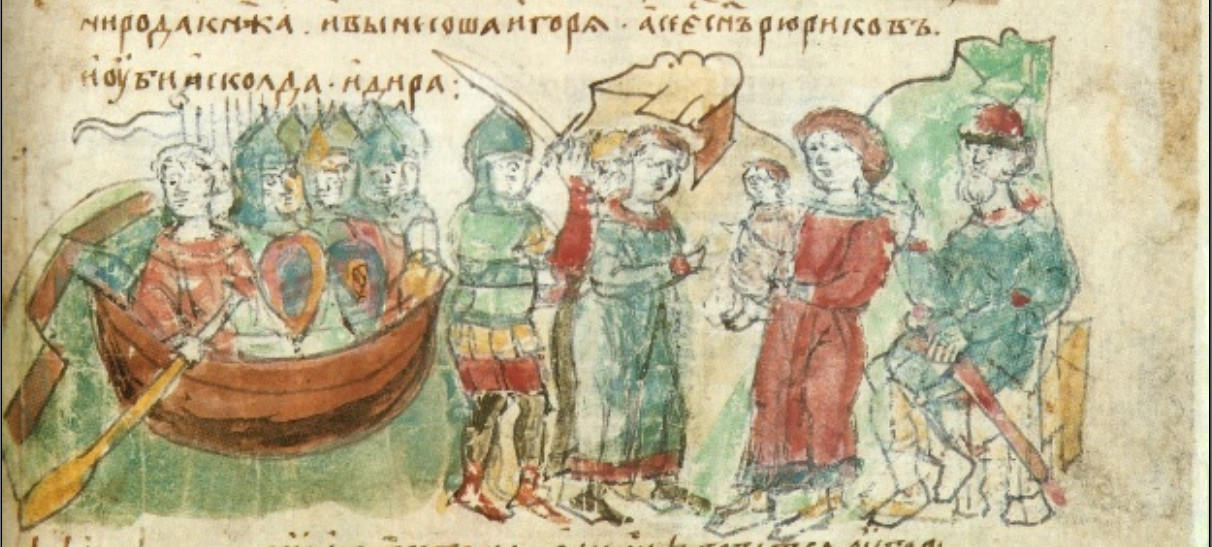
\includegraphics[width=\linewidth]{chast-volga/oskoldidir/radz-oskold.jpg}
\end{center}

Лаврентьевский список в подлиннике излагает это так:

\begin{quotation}
Поиде Олег поим вои свои многи варяги чюдь словени мерю вьсе кривичи и приде к смоленьску с кривичи и прия град и посади мужь свои отуда и поиде инизом взя Любец, и посади мужь свои 

придоста ко горам ко киевьскимь и оувиде Олег яко Осколдъ и Диръ княжита похорони вои в лодьях а другия назади остави а сам приде нося Игоря детьска

и приплу под Оугорьское похоронив вои свои и присла ко Асколду и Диру глаголя, яко «Гость есмь идем в Грекы от Олга и от Игоря княжича. Да придета к нам к родом своим». Асколд же и Дир придоста и выскакав же вси прочии из лодей, и рече Олег Асколду и Дирови: «Вы неста князя, ни роду княжа, но аз есмь роду княжа», и вынесоша Игоря: «а се сын Рюриков». 

И оубиша Асколда и Дира несоша на гору и погребоша и на горе, еже ся ныне зоветь Оугорьское, кде ныне Ольмин двор на той могиле поставил церковь святаго Николу а Дирова могила за святою Ориною. 

Седе Олег княжа в Киеве и рече Олег: «Се буди мти городом русским». Беша у него Словени и Варязи и прочи прозвашася Русью.

Се же Олег нача городы ставити, и устави дани Словеном, и Кривичем и Мерям, и устави Варягом дань даяти от Новагорода 300 гривен на лето, мира деля, еже до смерти Ярославле даяше Варягом.
\end{quotation}


По Ипатьевской летописи: 

\begin{quotation}
Поиде Олг поем вои свои многы Варягы Чюдь Словены Мерю Весь Кривичи и прия город и посади в нем мужь свои оттуда поиде вниз и пришед взя Любечь и посади мужь свои и прдоста к горам Киевьскым 

и оувиде Олг яко Осколд и Дир кнжита и похорони вои в лодьях а другыя назади остави а сам принося Игоря молоде и приступль под Оугорьское похоронив вои свои и посла к Асколду и Дирду гла яко гостье есмы идем к Грекы от Олга и от Игор княжича да приидта к роду своему к нам 

Аскольд же и Дирд придста и выскакаша вси из лодеи и ре Олг к Асколодови и Дирови в неста князя ни роду княжа но аз есмь роду кжа и вынесоша Игоря с сн Рюриков

и оубиша Аскольда и Дирда и несоша и на гору еже ныне зоветь Оугорьскои Олмин Двор на тои могиле поставил божницю стого Николы а Дирова могила за стою Ориною и седе Олег княжа в Кыеве и ре Олег се буди мт городо Рускым 

и беша оу него Словени и Врящи и прочии прозвашася Русью се же Олег начал городы стави и оустави Словен и Кривичем и Мерям и оустави Варяго дань даяти от Новагорода
\end{quotation}

Главные отличия – в Ипатьевской летопсии Игорь назван «молод» вместо «детеськ». Вся гора, где хоронят Аксольда, упомянута как «Оугорьскь Олмин Двор», что можно толковать как Угорский Олмин Двор, то бишь Олмин Двор именно в урочище Угорском, Угорский Олмин Двор, в отличие еще от некоего иного двора Олмы. Возможная разгадка пресловутого «Олмина» двора будет ниже, предвкушайте!

Также, на могиле Аскольда ставят не церковь, но божницу – что более логично, если могила язычника Аскольда это курган. Как на кургане поставить церковь? А вот маленькую божницу можно.

Теперь вспомним, что мы имеем дело с рукописями. Рукописи лежали в давних библиотеках не просто годами, десятилетиями, а веками. Их переписывали. Их правили и поверх текста, разные люди, в разное время, а затем эти правки переходили в другие списки, уже истолкованные переписчиками.

В подлиннике Ипатьевской летописи написано:

\begin{center}
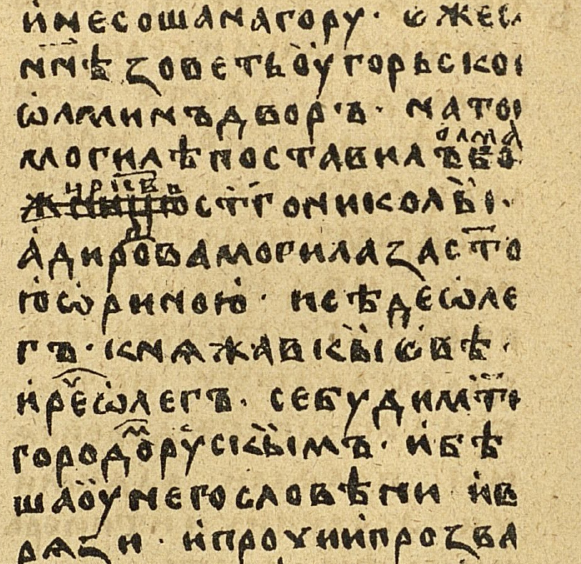
\includegraphics[width=\linewidth]{chast-volga/oskoldidir/MTI.png}
\end{center}

\begin{quotation}
и несоша на гору еже ныне зовется угорьскои олмин двор на той могиле поставил божницю святого николы [...]
\end{quotation}

«Божницу» перечеркнуто, и над «бо» стоит «олма». А далее над зачеркнутым «жницю» надписано «церковь». Смотрите сами:

Олма, Олма... Что если «м» то искаженная греческая буква «гамма»? таким образом получаем таки «Олга».

Возможно, некий писец употребил в написании имени «Олга», вместо славянской «г» греческую букву «гамма» – γ, которая кстати в заглавном виде имеет вид славянской «Г». 

Однако плоское, развесистое написание этой гаммы в виде эдаких бараньих рогов привело к ее трактовке как славянской «м». И возник загадочный Олма. Допустим, у исходного писца была такая особенность письма, причуда – кстати мы не знаем образца почерка Нестора. Далее я выпускаю из рассуждений Олму как отдельную личность и принимаю, что это иное написание Олга. Отмечу, что в некоторых списках вместо «Олма» или «Ольма» стоит таки «Олга». Однако есть чревоточина в моих рассуждениях про букву гамму, ее я представлю вам через несколько глав, и может статься, что Ольма или Олма тоже верное написание имени Олга и никакой гаммы тут нет.

...В иных списках Игорь не так беспомощен, и кроме прочего кланяется, бьет челом Олегу:

\begin{quotation}
И Ольг князь обманом призва к себе мужей тех Осколда и Дира. Они же, видевше со князем Ольгом мало людей, и изыдоша к нему на брег с великою частию и наченьше веселитися. И в то время внезапу прииде к ним немедленно Игорь княжичь со множеством без числа вои, челом ударя Олгу князю.
\end{quotation}

Игорь во главе части воинства – в списках не редкость:

\begin{quotation}
и возярися князь Олег и нача мыслити, коею бы виною мог уловити Асколда и и Дира.\footnote{Именно с двумя «и».} И собра воинство много в лодьях и на конех, а сам князь Олег поиде в лодиях в мале дружине, а Игоря княжича отпусти на конех со многим воинством.
\end{quotation}

Кстати, куда именно пристал Олег? В ряде списков, вместо привычного «под Оугорьское» – «под Киевец». О Киевце по спискам же известно, что «Кий з дружиною своею сотвори себе градец мал Киевец». Селение Киевец также было построено Кием где-то на Дунае, да местные его оттуда прогнали.

%Этот Киевец отделяется летописцем от Киевицы, горы, где поселился Кий. Есть Киевица гора, а где-то еще был построен Киевец. 

Киевец киевский упоминается обычно в списках новгородского толка, где Кий с братьями – разбойники из Новгорода, и вот они сподобились только на градец-Киевец, зато Олег «заложи град Киев великий» – заложил большую крепость Киев, б\'ольше прежнего града (крепости) Киева. Снова не указывается впрочем, где именно.

Таким образом по новгородским спискам история Киевщины приземляется и укорачивается. Вместо князей, на равных общавшихся с царьградским василевсом – бандиты, свившее себе на холмах гнездо Киевец. Где он был, неясно. На Угорьском?

Обычно таких вопросов не задают, полагая, что Олег пристал к берегу горы под будущей Аскольдовой могилой. Как-то само собой разумеется! Сказано ведь в более известных списках не про Киевец, но – «и приплыл под Оугорьское». Угорьское же относят к горе около Аскольдовой могилы. Исходя из соображений, которые я изложу позже, там же и был, при Аскольде с Диром и по крайней мере по Мономаха, княжий двор. Где же еще сидеть Аскольду с Диром, они ведь правители! Но...

%Что же получается? По малоизвестным спискам Олег приплыл под Киевец. По более известным – под Угорьское. В иных место умалчивается, либо так – Олег представляется как «гость есмь Подугорский, и иду в Греки от Олга князя и от Игоря княжича». А если тут зацепка? Олег не причалил к Угорьскому, но назвался гостем «подугорским»? Уграми именовали Венгров, Мадьяр – может, Олег имеет это в виду, либо нечто другое, я не знаю.

Под нынешнюю Аскольдову могилу, с которой соотносят «Угорьское», Олег не мог добраться незамеченным и осуществить свою хитрую задумку! %Важная оговорка – это ежели населенный тогда Киев располагался в привычном нам «старом городе».

Откуда пришел Олег к Киеву? От Любеча. Любеч находится на левом берегу Днепра, в 137 километрах выше Киева. При движении оттуда на юг, к «горам Киевским», да еще с конницей, Олегу надо было, во-первых, переправиться на правый берег. Во-вторых, дабы пристать к местности, что потом прослыла Аскольдовой могилой, Олегу требовалось незаметно провести лодьи и конницу мимо трех «княжеских» гор – Хоревицы, Щекавицы и Киевицы. Ведь Аскольдова могила их южнее.

Как же так? Может, Олег с войском сделал большой крюк, добирался под будущую Аскольдовку некими протоками, а ранее у Вышгорода переправил конницу на правый берег, незаметно\footnote{Сдавленный кашель.} провел к городу и вокруг него... Но была ли конница? Какому списку верить?

Конница делает место действия – Угорьское (современная Аскольдова могила) невозможным. Либо место действия делает невозможной, выдуманной конницу.

А допустим, Олег пристал не под место, слывущее ныне Аскольдовой могилой. Но куда?

Вспомним, где на миниатюре Радзивилловской летописи показан «град Киев» при Кие, Хориве и Щеке. В районе Кирилловских высот, на тамошней Лысой горе, слывущей ныне Юрковицей. В этом случае Олег просто подошел бы туда с севера, а лодьи можно было пустить Почайной.

В рукописи поручика Василия Ивановича Новгородцева «Географическое описание Киева», 1784 года\cite{sbornikmat}, вдруг находим среди описания отделений города (Андреевского, Печерского, Софийского, Михайловского, Печерского) такое:

\begin{quotation}
1-е. Андреевское отделение можно полагать за начало и распространение Киева [...] думать надобно, что гора Зборичев есть та самая, где апостол Андрей крест поставил; почему ныне и называется Андреевское отделение, а укреплено оное земляным валом.

Дира могила насыпанная бугром и поныне находится в разстоянии от Стараго Киева в 3-х верстах недалеко от Кириловского монастыря. На оном месте была церковь деревянная Воздвижения креста Господня которая около 1725 комендантом Поросуковым сломана, а в 1744 году на оном месте заложена  каменная церковь во имя апостола Андрея Первозваннаго.
\end{quotation}

Первое предположение противоречит второму. Мол, могила Дира была недалеко от Кирилловского монастыря. А далее Новгородцев дополняет – на оном месте была церковь деревянная и так далее, говоря об Андреевской горке!

В 1701 старец Леонтий, посетивший Киев, записал, что на холме, где по преданию апостол Андрей водрузил (в 40 году нашей эры) крест, стоит деревянная и ветхая церковь во имя святого апостола Андрея Первозванного. 

До знаменитой Андреевской церкви архитектора Растрелли была там одноименная деревянная. Еще ранее, в 1212 году, где-то в том же месте, Мстислав Романович поставил Крестовоздвиженскую церковь – о ней Новгородцев и пишет: «Воздвижения креста Господня». Однако ее, по словам Закревского и Похилевича, разрушили в 1240 году, при взятии Киева ханом Батыем. И никто толком не ведает, где именно она была, только Похилевич со знанием дела пишет – в нескольких десятках саженях от Андреевской. Какую же церковь сломал комендант Поросуков?

Но оставим Крестовоздвижескую. Внимательно посмотрим на текст Новгородцева. Кажется, что слова про Дирову могилу в нем лишние, вставленные по ошибке. И «на оном месте» следует считать относящимся к горе, где апостол Андрей крест поставил, а не трактовать, что на месте Дировой могилы был крест и потом две церкви.

Предложение «Дира могила насыпанная бугром и поныне находится в разстоянии от Стараго Киева в 3-х верстах недалеко от Кириловского монастыря» здесь чуждое. Но его надобно рассматривать отдельно, как утверждение, что могила Дирова расположена поблизости Кирилловского монастыря.

В предыдущей части книги много сказано о курганах Кирилловских высот – курганы там были, а вероятно некоторые еще целы. Сведения о Дировой могиле именно в районе Кирилловских высот – весомый довод в пользу предположения, куда пристал Олег и где находился град Киев. Не местность ли под названием Курган, с пещерой внутри (подробности в части про Логово Змиево), слыла могилой Дира?

Вступает ли это в противоречие с расположением Аскольдовой могилы? Нет. Убили в одном месте, похоронили в другом. Противоречие будет в случае, если Олег прибыл под Угорьское, к Аскольдовке и Берестовому. Но добраться туда с севера, проплыв мимо холмов Кия, Хорива и Щека, да еще протащив тайно конницу Игоря, Олег не мог физически.

Возможны следующие варианты решения задачи, с той или иной натяжкой.

Первый – в основных списках ошибка, Олег пристал не под Угорьское, но много севернее. Конницу обычно подводили со стороны Лыбеди либо Дорогожичей. Последние соседствуют с Кирилловскими высотами.

Второй – Олег пристал таки под Угорьское, потому что эта местность и была местом обитания князей, «столом».

Княжеский престол в окрестностях Угорьского и Берестова – данность, отраженная в летописях, на первых порах Киевской Руси. Сие мы обсудим позже.

Но применительно ко времени Аскольда и Дира это должно означать, что местность выше по течению – а именно Кирилловские высоты и Киевица (Старокиевская гора), по какой-то причине пустовали, во всяком случае княжий двор находился не там.

Нестор пишет, что убили Аскольда и Дира, и «несоша на гору» – обоих ли, одного ли? Далее изложение в основных летописях различно. По Лаврентьевской, «и погребоша и на горе» – то есть погребли его на горе, «Оугорьско Олмин Двор», «и на той могиле поставил церковь святаго Николу, а Дирова могила за святою Ириною».

«Несоша на гору» – не обязательно на место захоронения. Просто – куда-то наверх. Ведь убили – внизу, у берега. И на горе, которая при Несторе именуется Угорьский Олгин двор, или просто Угорьское, погребли Аскольда. А могила Дира – за святой Ириной.

А в Ипатьевской летописи рассказано без погребения: «и несоша на гору, еже ся ныне зовет Угорьскои Олмин двор». Читаешь и невольно думаешь – значит, там и похоронили, хотя летопись об этом молчит.

На могиле Аскольда, «Олма» ставит церковь святого Николая.
 
Угорьское – это урочище, гора, один из склонов Днепра, имя получивший вот почему, согласно Ипатьевскому списку:

\begin{quotation}
Идоша Угре мимо Киева горою, еже ся зовет ныне Угорьское, и, пришедше к Днепру сташа вежами.
\end{quotation}

Также могу предположить, что «Угорьское» означает просто «у горы». По летописным сведениям, Угорськое было смежным с Днепром и такими местностями, как Берестово и Клов, там же стояли некие Угорьские ворота. Возле Угорьского было достаточно места для народных собраний. Согласно Закревскому, даже в 19 веке киевляне называли урочище близ Аскольдовой могилы «Угорським». 

%В Ипатьевской летописи, о годе 1151-м, упомянуты также «Угорския ворота» и «княжий двор» относительно этой местности. 

% В Ипатьевской летописи за 1146 (6654) год сказано про Игоря Ольговича\footnote{Вскоре Игоря заточат в поруб, а спустя год те же Кияне потащат избитого князя голым на веревке через Бабин Торжок на княжий двор, где прикончат его.}: 

%\begin{quotation}
%и пояша (Кияне) Игоря в Киев, иде с ними под Угорьский, и съзва Кияне вси; они же вси целоваше к нему крест, рекуче: «ты нам князь».
%\end{quotation}

Сейчас однозначно решить задачу про Угорьское и его отношение к убийству Олегом киевских князей нельзя. Учитывая, что ранее, при покорении Смоленска, Олег – по некоторым спискам – встал у города выше по течению и тоже предъявил горожанам Игоря, можно полагать, что в Киеве он, хотя и подло, проделал то же самое – и убийство с предъявлением «настоящего князя» состоялось у Кирилловских высот либо чуть севернее. И Дира похоронили там же, а Аскольда – южнее, на Угорьском.

Еще вариант летописный, поздний, судя по языку изложения:

\begin{quotation}
Олег показал им Игоря Руриковича, глаголя: яко сей есть Наследник всех Княжений Российских сын Руриков; и абие повеле Осколда и Дира пред собою побити; и погребоша Осколда на горе, на нейже потом Великая Княгина Ольга окрестившая первую церковь святаго Николы в Киеве постави, а Дирова могила за церквою святыя Ирины.
\end{quotation}

Берлинский сообщает – без ссылки на источник, что:

\begin{quotation}
В 969 году по преставлении своем Блаженная Княгиня Ольга, была погребена в сей Ольмовой церкви, откуда потом внук ея велю Князь святой Владимир перенес ея в новосозданную Десятинную церковь.
\end{quotation}

Место захоронения княгини Ольги – вопрос, которого мы еще коснемся. А вот Максимович склонялся к мысли, что церковь святого Николая была построена таки княгиней Ольгой, в пользу чего приводил размышление – мол, при церкви был именно женский монастырь. Монастырь этот существовал уже при Несторе, в 10 веке, а в 12 стал мужским.

Олг, Ольга, Олм, Олма и так далее. Путаница! Возникает из рукописной природы летописей и традиционной трактовки истории. Как толковать иначе, и проще, и понятнее, и удивительнее, вы узнаете в следующих главах. 

Пока задаток. Противоречия устранятся, как только мы примем Вещего Олега и княгиню Ольгу за одно лицо!

Вещий Олег (Олг, Ольг, Олга), он же в будущем княгиня Ольга (Олга), устроил около Берестове свой княжий двор. Потому при Несторе там же «Олгин двор».

%Вещий Олег носил в народе усредненное, бесполое имя Вольга, что произносилось скорее как Волха, Вольха.

Но ключ к пониманию летописных выражений лежит в окончаниях имен при родительном падеже. Мужское имя Олг склоняется так – Олгов двор. Женское Олга склоняется – Олгин двор. «Ольмин двор» из Лаврентьевской летописи указывает на женский род имени. Почему вместо Ольга некоторые списки пишут Ольма, я расскажу через три главы. Это равнозначные имена, и Нестор по сути говорит, что в его время гора Угорьское носит второе название – Ольгин двор.

В той же летописи, именно Олег хоронит там Аскольда и, язычник, воздвигает христианскую церковь. Полагаю, источник, коим пользовался Нестор, не путал Олега с Ольгой, приписывая то ему, то ей заложение церкви Николая. Запутали позже – сам Нестор либо позднейшие переписчики, сделав из одной личности две.

Но где возвели храм? В те времена их не строили на отшибе – опасно! Значит, в черте города либо в пределах защищенного монастыря. Поскольку гора прослыла Олгиным или Олминым двором, предположу, что этот «двор» и служил укреплением, под защиту которого попадала церковь, если только вся местность не входила в городскую черту, за крепостной стеной.

Угорьское по летописям вовсе не выглядит окраиной. А с ним совмещается или соседствует знаменитое Берестове, которое считают загородным имением князей. 

Верно ли такое мнение?
